\renewcommand{\theequation}{\theenumi}
\begin{enumerate}[label=\arabic*.,ref=\thesubsubsection.\theenumi]
\numberwithin{equation}{enumi}

\item In the given question,
\\
The sample size = Total Area of the rectangle=
\begin{align}
3x2=6 m^2
\end{align}
Favourable outcome = Area of Circle=
\begin{align}
\pi\brak{\frac{1}{2}}^2=\frac{\pi}{4} m^2 
\end{align}
Probabilty(P) of the dice landing in the circle=$\frac{\pi}{24}$
\\
$\therefore$ P = 0.1308
\\
The python code for the figure \ref{fig:figure}
\begin{lstlisting}
prob/codes/prob1.py
\end{lstlisting}
shows the histogram plot data in 1000 dice throws.
\begin{figure}[!ht]
\centering
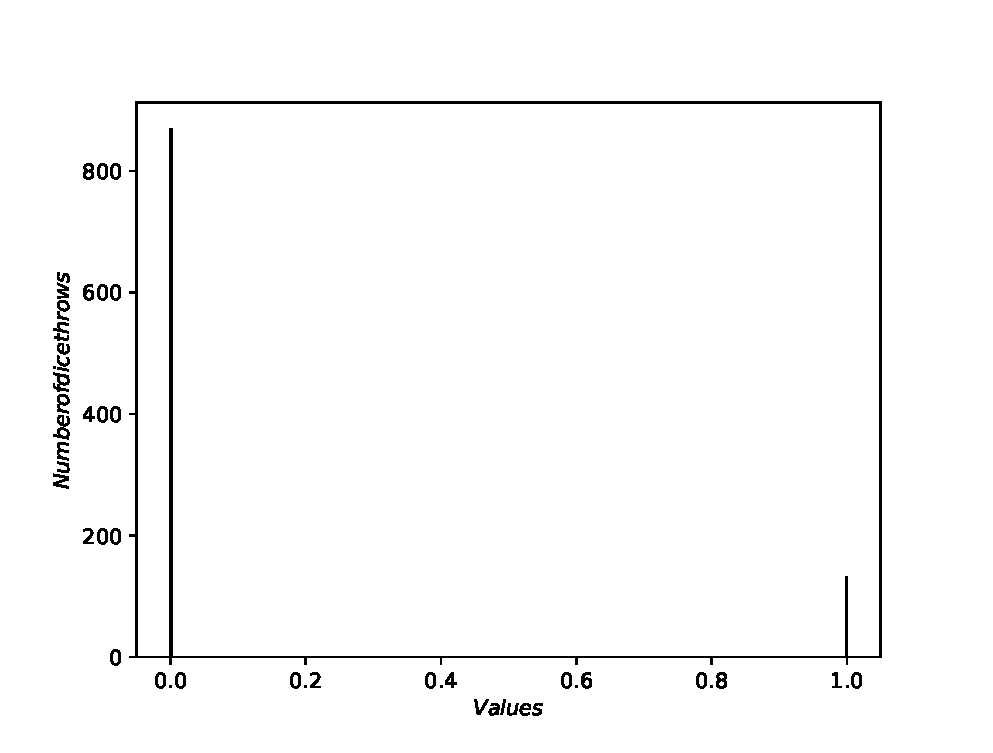
\includegraphics[width=\columnwidth]{./prob/figs/prob1.eps}
\caption{Histogram}
\label{fig:figure}
\end{figure}
\\
The Value 0 in the figure \ref{fig:figure} shows that out of 1000 throws 869 times, it doesn't fall in the circle, for the rest of 131 throws the dice is in the circle.
\end{enumerate}